% !TEX root = knauss-vissuelizer.tex
\section{Example Scenarios}
In this section we describe examples that highlight the functionality of the \viss\ tool.

\subsection{Where are the hotspots in a set of issues?}
\begin{figure}[b]
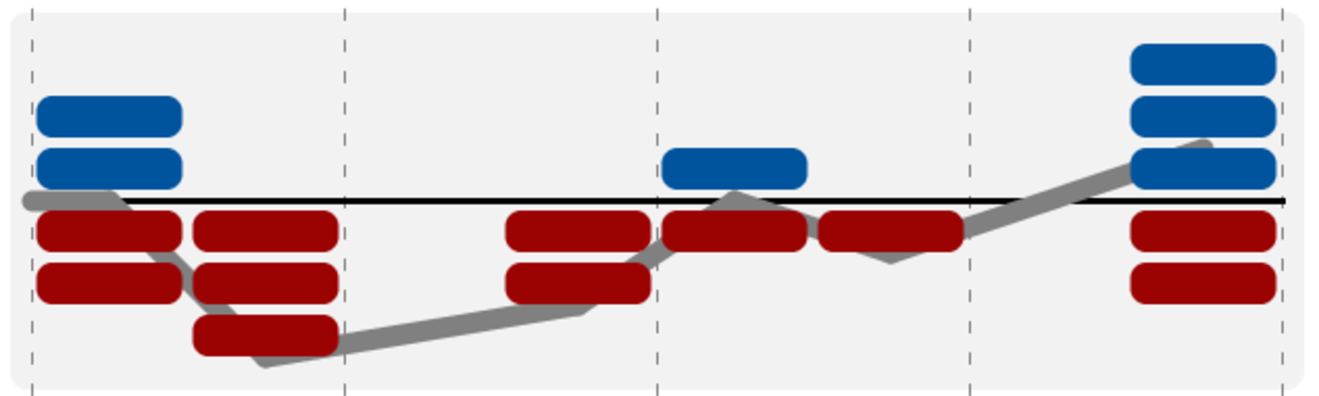
\includegraphics[width=\columnwidth]{img/example-trajectory}
\caption{Example of a requirements discussion's clarification trajectory}
\label{fig:example-trajectory}
\end{figure}
Often, a clear understanding of requirements only evolves during the development of software.
This is especially true (but not limited to) agile software projects, where managers decide to frame only rudimentary requirements and refine the details on the go.
For a manager, it is important to know when problematic requirements surface, because they can have a serious impact on the project.
\viss\ helps managers in this scenario as follows:
\begin{enumerate}
\item The manager loads a set of requirements (e.g. user stories for the current iteration).
\item \viss\ automatically analyzes the discussion events that are related to these requirements and that are available in online communication.  
\item \viss\ creates a set of \emph{clarification trajectories} (c.f. Figure \ref{fig:example-trajectory}), one for each requirement. 
%Discussion events that are concerned with clarifying requirements are depicted by red rectangles below the timeline, other comments are depicted by blue rectangles above the timeline.
\item \viss\ also displays suggestive pattern names for distinctive trajectories (e.g. textbook-example, back-to-draft, procrastination).
\item The manager scrolls through the requirements and associated trajectories and decides based on this rich information where to invest more resources.
\end{enumerate}
Typically, there is a number of requirements without pathological findings, e.g. user stories with some clarification in the beginning and other communication events later on that show progress. 
But there are also suspicious trajectories, e.g. a large amount of clarification late in the iteration, perhaps even after the issue seemed to be solved, or no clarification at all, even though the requirement seems to be complex.

\subsection{Are there any communication breakdowns?}
After identifying those hotspots, the manager most likely wants to continue with a closer investigation. 
Often, he or she will investigate who participates in a discussion of a requirement and who is not.
\begin{enumerate}
\item The manager opens the social network analysis view.
\item \viss\ creates the social network for the selected requirement.
\item The manager analyzes the network and investigates if structural communication problems exist.
\end{enumerate}

\begin{figure}
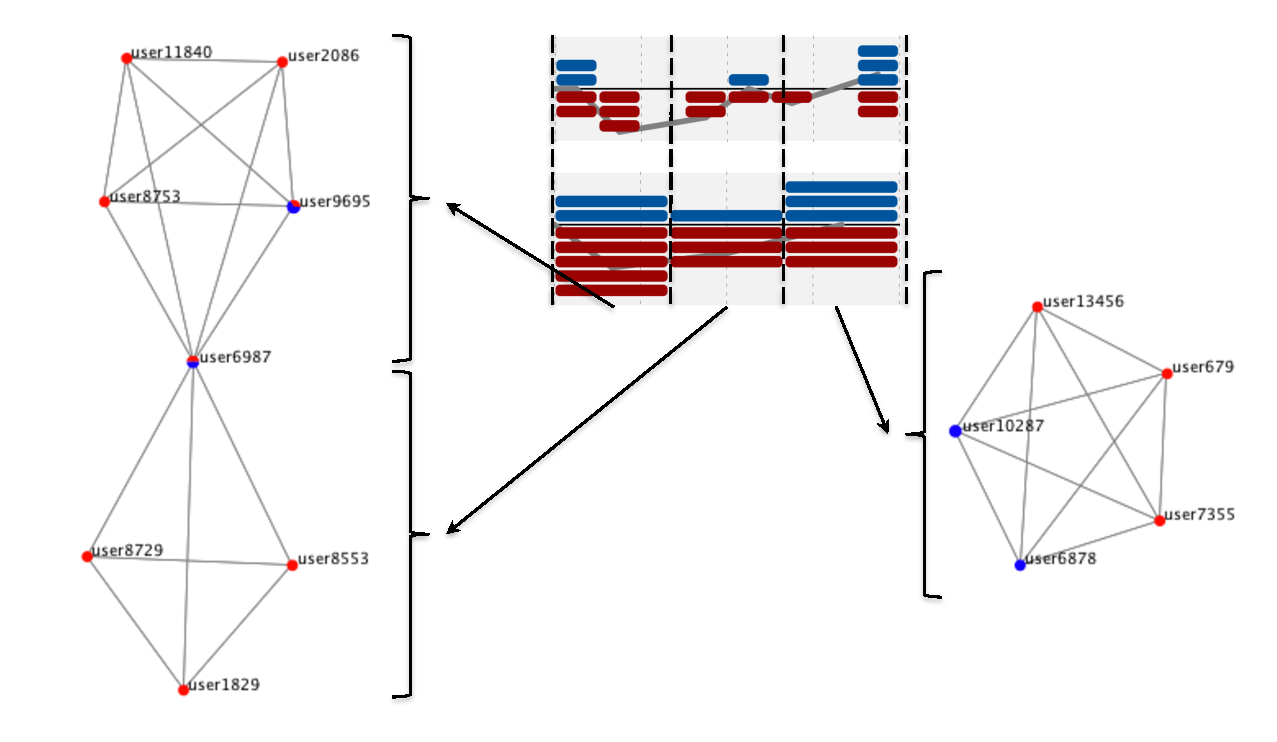
\includegraphics[width=\columnwidth]{img/example-sn}
\caption{Example of a requirements discussion's social network}
\label{fig:example-sn}
\end{figure}

In the example above, the manager might conclude that there is no single person who is coordinating the analysis and work around this requirement, because there is no actor who participates in all relevant time intervals.
A suitable action might be to assign this responsibility to a more experienced developer.

\subsection{Who is knowledgeable about a given topic?}

Integrating the right persons in the loop for an important feature is a crucial ability for managers.
\begin{enumerate}
\item The manager selects a number of requirements that are related to a given topic. 
\item \viss\ integrates the social networks of these requirements discussions in a single large network (see Figure \ref{fig:example-sn-large}).
\item The manager uses the pie charts in the social network to determine, which candidate has a balanced percentage of clarification and other communication.
\item The manager looks for central developers. 
\end{enumerate}
\begin{figure}
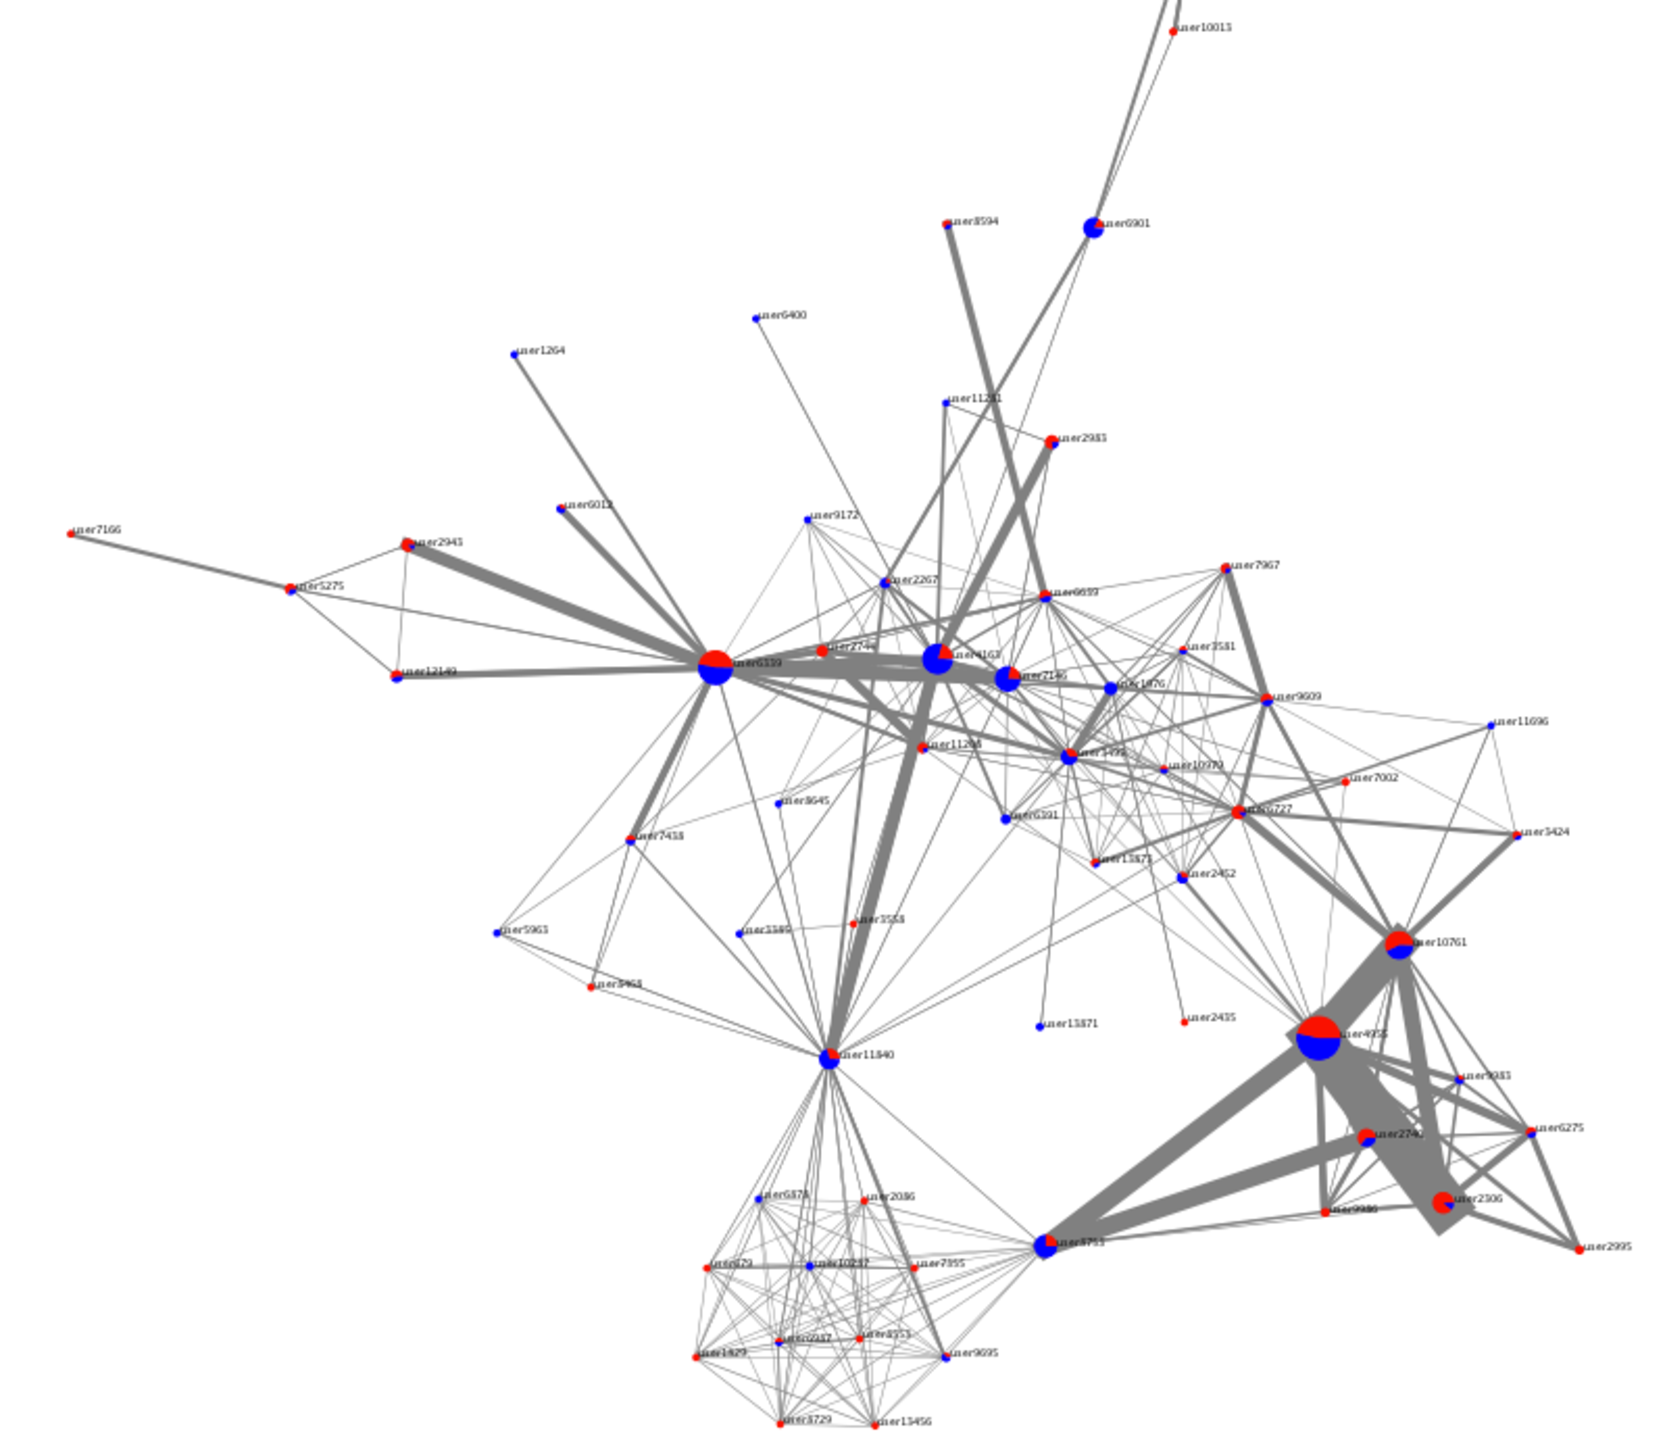
\includegraphics[width=\columnwidth]{img/example-sn-large}
\caption{Example of a social network for a set of requirements discussions}
\label{fig:example-sn-large}
\end{figure}
Central actors with many connections might already have a very high workload, but there exist good candidates that are less central and connect two subnets.
